\documentclass {article}

\usepackage[utf8]{inputenc}
\usepackage{graphicx}
\usepackage{listings}
\usepackage{color}
\usepackage{float}

\definecolor{dkgreen}{rgb}{0,0.6,0}
\definecolor{gray}{rgb}{0.5,0.5,0.5}
\definecolor{mauve}{rgb}{0.58,0,0.82}

\lstset{frame=tb,
    language=C,
    aboveskip=3mm,
    belowskip=3mm,
    showstringspaces=false,
    columns=flexible,
    basicstyle={\small\ttfamily},
    numbers=left,
    numberstyle=\tiny\color{gray},
    keywordstyle=\color{blue},
    commentstyle=\color{dkgreen},
    stringstyle=\color{mauve},
    breaklines=true,
    breakatwhitespace=true,
    tabsize=3
}


\title{Rapport projet laboratoire M1\\
Programmation parallèle pour réseau de neurones }
\date{\today}
\author{ABDELMOUMENE Djahid}

\begin{document}
\maketitle
\newpage


\section{Introduction}
Dans ce projet nous essayons de tester plusieurs techniques d'optimisation parallèle, et éventuellement les mettre en œuvre sur un implementation d'un bibliothéque des réseaux neurones.

\section{Les techniques d'optimisation utilisé}
\subsection{Algorithme naive}
Nous prenons comme point de référence l'algorithme naïf avec trois boucles imbriquées:

\begin{lstlisting}
for(i=0; i<N; i++) {
    for(j=0; j<N; j++) { 
        acc = 0.0;
        for(x=0; x<N; x++) {
            acc += a[i][x] * b[x][j];
        }
        res[i][j] = acc;
    }
}
\end{lstlisting}


\begin{figure}[H]
    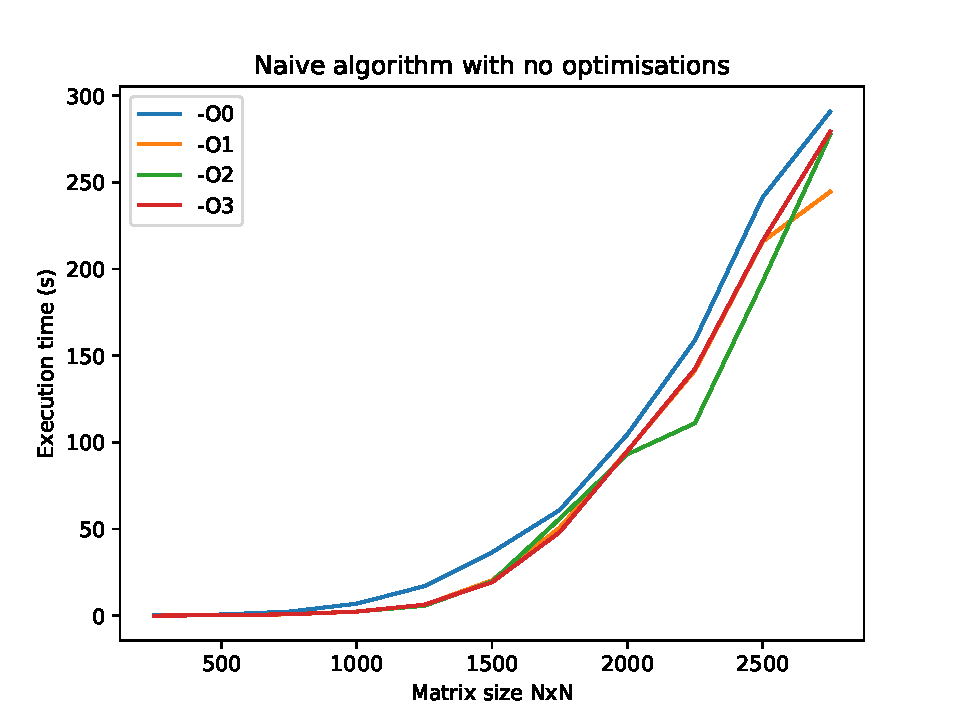
\includegraphics[width=\linewidth]{plot/no_opt.pdf}
    \caption{Pas d'optimisations}
    \label{fig:no_opt}
\end{figure}

Ce que nous pouvons remarquer ici, c'est que l'effet des niveaux d'optimisation de GCC commence à faiblir quand N devient de plus en plus grand.

\subsection{Optimisations de boucles imbriquées}
Pour les optimisations 
\begin{lstlisting}
int ib = 10, kb = 10;
for (ii = 0; ii < N; ii += ib) {
    for (kk = 0; kk < N; kk += kb) {
        for (j=0; j < N; j += 2) {
            for(i = ii; i < ii + ib; i += 2 ) {
                if (kk == 0)
                acc00 = acc01 = acc10 = acc11 = 0;
                else {
                    acc00 = res[i + 0][j + 0];
                    acc01 = res[i + 0][j + 1];
                    acc10 = res[i + 1][j + 0];
                    acc11 = res[i + 1][j + 1];
                }
                for (k = kk; k < kk + kb; k++) {
                    acc00 += b[k][j + 0] * a[i + 0][k];
                    acc01 += b[k][j + 1] * a[i + 0][k];
                    acc10 += b[k][j + 0] * a[i + 1][k];
                    acc11 += b[k][j + 1] * a[i + 1][k];
                }
                res[i + 0][j + 0] = acc00;
                res[i + 0][j + 1] = acc01;
                res[i + 1][j + 0] = acc10;
                res[i + 1][j + 1] = acc11;
            }
        }
    }
}
\end{lstlisting}

\begin{figure}[H]
    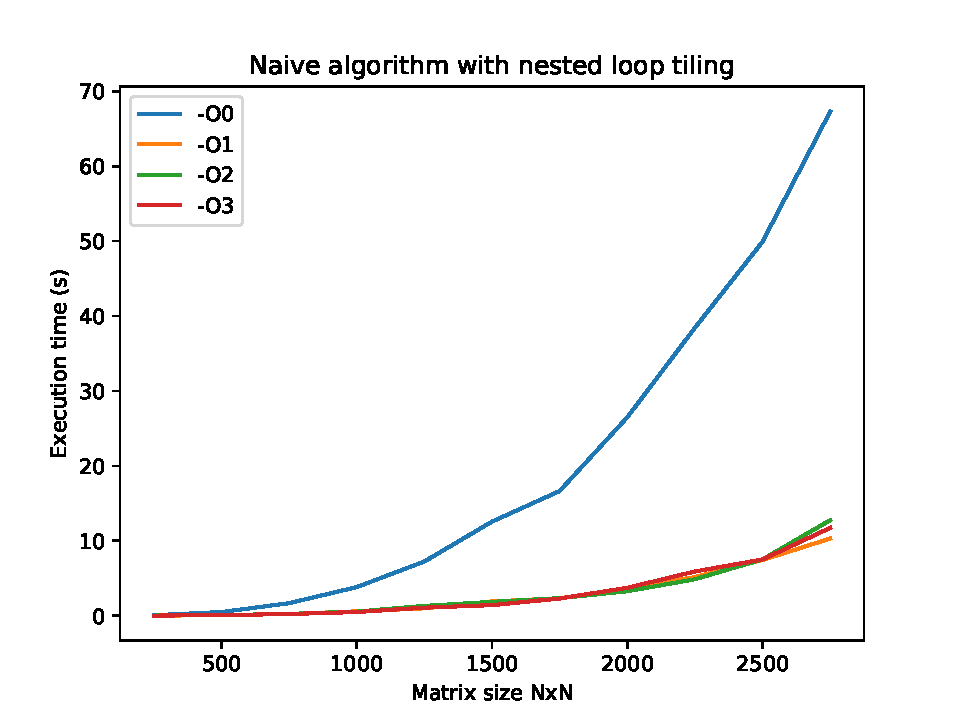
\includegraphics[width=\linewidth]{plot/with_opt.pdf}
    \caption{Avec les optimisations}
    \label{fig:with_opt}
\end{figure}

\subsection{Parallélisation}

\begin{lstlisting}
#pragma omp parallel for shared(a, b, res) \\
                         private(i, j, x, acc) \\
                         schedule(static)
for(i=0; i<N; i++) {
    for(j=0; j<N; j++) { 
    acc = 0.0;
    for(x=0; x<N; x++) {
        acc += a[i][x] * b[x][j];
    }
    res[i][j] = acc;
    }
}
\end{lstlisting}

\begin{figure}[H]
    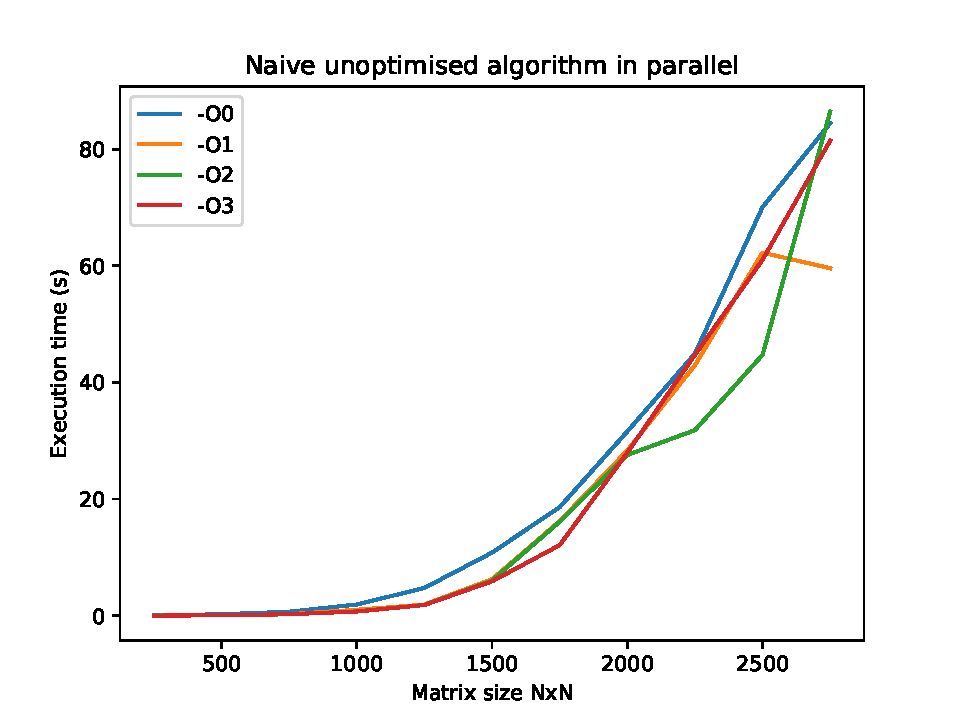
\includegraphics[width=\linewidth]{plot/parallel.pdf}
    \caption{Exécuté en paralléle}
    \label{fig:parallel}
\end{figure}

\subsection{Optimisations et parallélisation}

\begin{lstlisting}
int ib = 10, kb = 10;
#pragma omp parallel for shared(a, b, res, ib, kb) \\
              private(i, ii, j, k, kk, acc00, acc01, acc10, acc11) \\
              schedule(static)
for (ii = 0; ii < N; ii += ib) {
    for (kk = 0; kk < N; kk += kb) {
        for (j=0; j < N; j += 2) {
            for(i = ii; i < ii + ib; i += 2 ) {
                if (kk == 0)
                    acc00 = acc01 = acc10 = acc11 = 0;
                else {
                    acc00 = res[i + 0][j + 0];
                    acc01 = res[i + 0][j + 1];
                    acc10 = res[i + 1][j + 0];
                    acc11 = res[i + 1][j + 1];
                }
                for (k = kk; k < kk + kb; k++) {
                    acc00 += b[k][j + 0] * a[i + 0][k];
                    acc01 += b[k][j + 1] * a[i + 0][k];
                    acc10 += b[k][j + 0] * a[i + 1][k];
                    acc11 += b[k][j + 1] * a[i + 1][k];
                }
                res[i + 0][j + 0] = acc00;
                res[i + 0][j + 1] = acc01;
                res[i + 1][j + 0] = acc10;
                res[i + 1][j + 1] = acc11;
            }
        }
    }
}
\end{lstlisting}

\begin{figure}[H]
    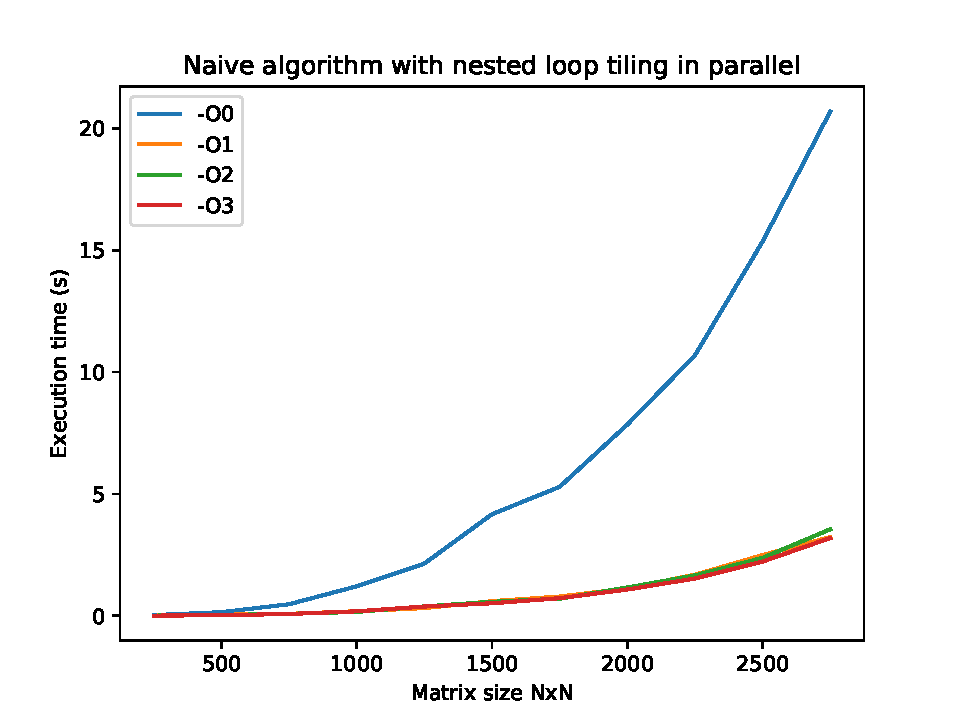
\includegraphics[width=\linewidth]{plot/with_opt+parallel.pdf}
    \caption{Avec les optimisations et en paralléle}
    \label{fig:with_opt+parallel}
\end{figure}
\section{Comparaison entre les algorithmes}
\begin{figure}[H]
    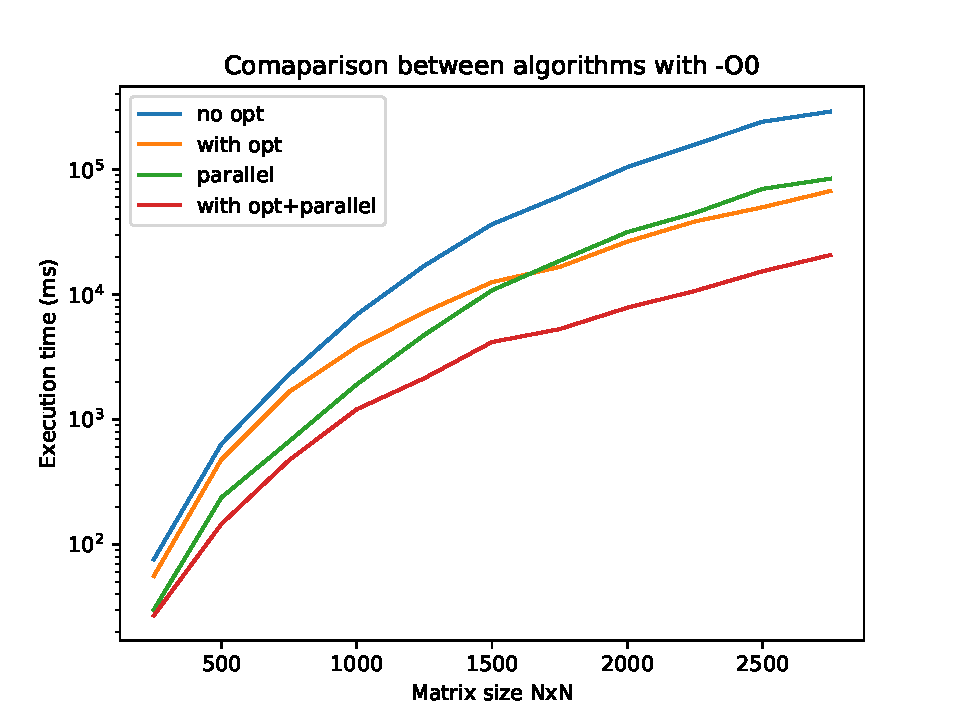
\includegraphics[width=\linewidth]{plot/compare_O0.pdf}
    \caption{Avec niveau d'optimisation 0 (échelle logarithmique)}
    \label{fig:compare_O0}
\end{figure}

\begin{figure}[H]
    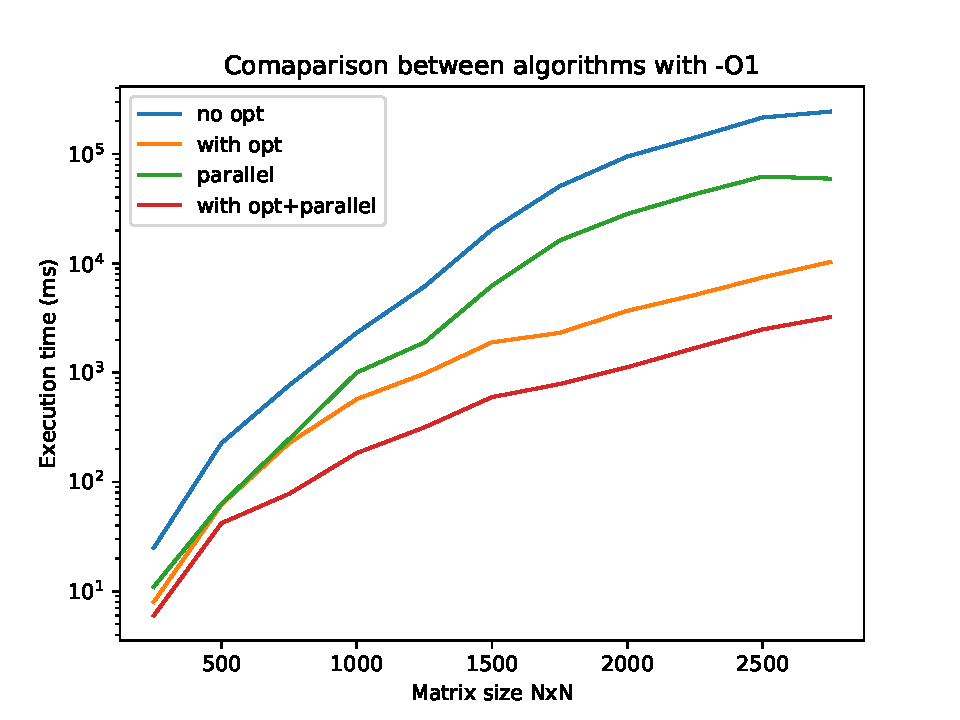
\includegraphics[width=\linewidth]{plot/compare_O1.pdf}
    \caption{Avec niveau d'optimisation 1 (échelle logarithmique)}
    \label{fig:compare_O1}
\end{figure}  

\begin{figure}[H]
    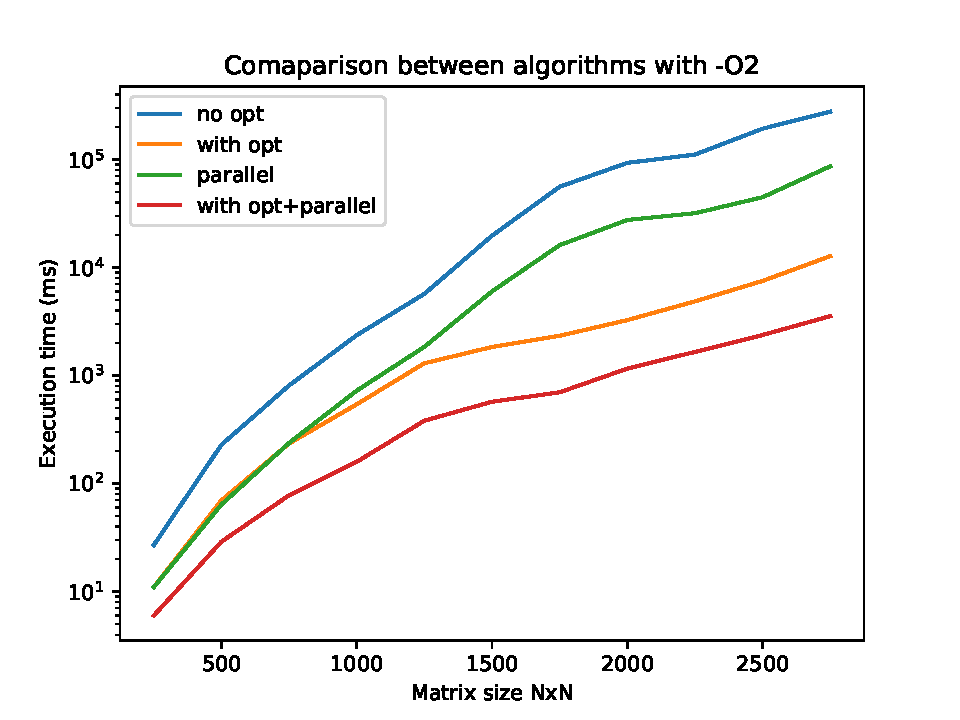
\includegraphics[width=\linewidth]{plot/compare_O2.pdf}
    \caption{Avec niveau d'optimisation 2 (échelle logarithmique)}
    \label{fig:compare_O2}
\end{figure}

\begin{figure}[H]
    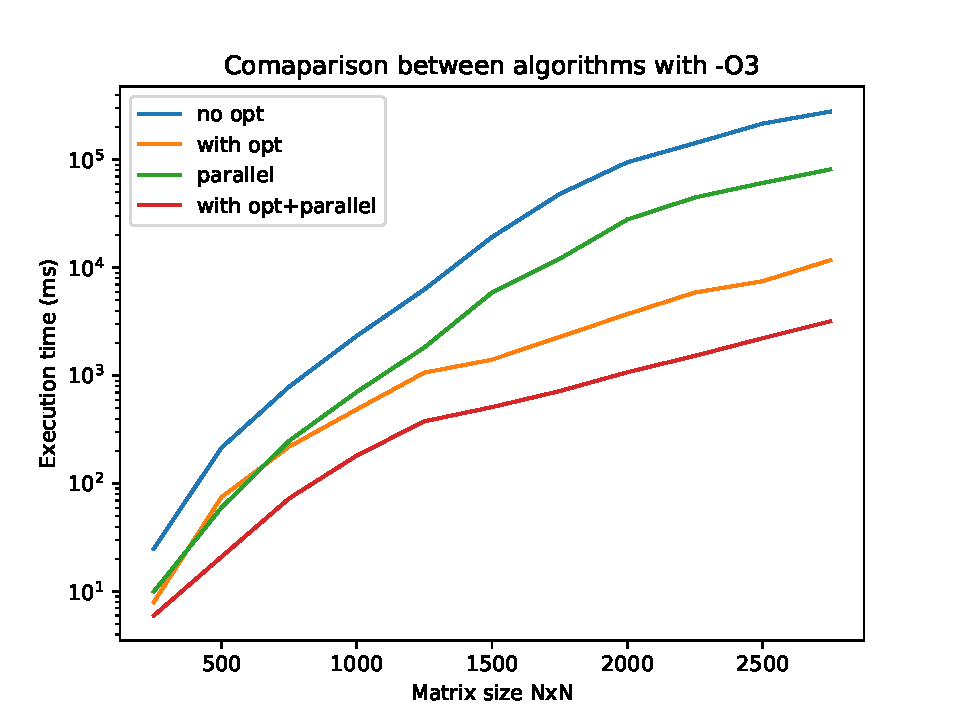
\includegraphics[width=\linewidth]{plot/compare_O3.pdf}
    \caption{Avec niveau d'optimisation 3 (échelle logarithmique)}
    \label{fig:compare_O3}
\end{figure} 
\section{Observations}

\end{document}
